% This work is licensed under the Creative Commons
% Attribution-NonCommercial 3.0 Unported License. To view a copy of this
% license, visit http://creativecommons.org/licenses/by-nc/3.0/.

\section{Theorie}
\subsection{Natur des Lichts}
%
Licht kann in diesem Versuch als elektromagnetische Welle 
beschrieben werden.\\
Dieses besteht aus einem elektrischen und einem magnetischen Anteil, 
welche direkt voneinander abhängen. Deswegen reicht die Betrachtung 
des elektrischen Anteils aus.\\
Des weiteren breitet sich Licht im Vakuum immer mit 
Lichtgeschwindigkeit aus.\\
Da in diesem Versuch ein Helium-Neon-Laser verwendet wird, 
reicht die Betrachtung von monochromatischen Licht, d.h. Licht 
mit nur einer Wellenlänge, aus. Der elektrische Wellenanteil des 
monochromatischen Lichtes kann also durch die in 
Gleichung~\eqref{eq:welle} angegebene Funktion von 
Raum und Zeit mathematisch ausgedrückt werden.
%
\begin{equation}
\vec{E}(\vec{r},t) = \vec{E_0}\cdot \exp{(i(\omega\cdot t - 
\vec{k}\cdot \vec{r}))}
\label{eq:welle}
\end{equation}
%
Die elektrische Welle ist ein Vektor.
$\vec{E_0}$ gibt die Polarisation des Lichtes an. In diesem Versuch 
wird mit linear polarisiertem Licht gearbeitet, d.h. $\vec{E_0}$ ist 
konstant.\\
Bei Wellen tritt das Phänomen der Interferenz auf. Dabei 
addieren sich die Wellenvektoren in jedem Raumzeitpunkt.
Aufgrund der Linearität der Maxwellgleichungen führt diese Operation 
zu einer Funktion, die ebenfalls die Maxwellgleichungen erfüllt.\\
Es folgt eine Rechnung zur Beobachteten Intensität zweier 
interferierender Wellen.\\
Sei der elektrische Wellenanteil des ersten Strahls gegeben durch
\begin{equation}
\vec{E_1} = \vec{E_{01}}\cdot \exp{(i(\omega\cdot t - 
\vec{k}\cdot \vec{r}))}.
\end{equation}
Der zweite Strahl besitze eine andere Polarisation und Amplitude.
Der Winkel zwischen den beiden Polarisationsachsen werde mit 
$\delta$ bezeichnet.
Außerdem besitze dieser eine Phasenverschiebung zum ersten von 
$\phi$. Die zweite Welle wird also durch
\begin{equation}
\vec{E_2} = \vec{E_{02}}\cdot \exp{(i(\omega\cdot t - 
\vec{k}\cdot \vec{r} + \phi))}
\end{equation}
beschrieben.\\
Die beobachtete Intensität ergibt sich also zu
\begin{equation}
I \propto \left<\left|\vec{E_1}+\vec{E_2}\right|^2\right>
=E_{01}^2 + E_{02}^2 + 2E_{01}E_{01}\cos{(\delta)}\cos{(\phi)}.
\label{eq:intense}
\end{equation}
Bei gleicher Polarisation, also bei $\delta =0$ sind die Fälle der 
destruktiven und konstruktiven Interferenz leicht zu sehen.
\begin{align}
\phi = \pi : I\propto E_{01}^2 + E_{02}^2 - 2E_{01}E_{02} 
 = 0 \text{ für } E_{01}=E_{02}\\
\phi = 0 : I\propto E_{01}^2 + E_{02}^2 + 2E_{01}E_{02} 
 = 4E_{01}^2 \text{ für } E_{01}=E_{02}
\end{align}
Stehen die Polarisationsrichtungen der beiden Lichtstrahlen hingegen 
senkrecht aufeinander, ist also $\delta = \pi/2$, so ergibt sich
\begin{equation}
I \propto E_{01}^2 + E_{02}^2.
\end{equation}
Bei senkrecht zueinander polarisiertem Licht tauchen also keine 
Interferenzeffekte auf!
%
\subsection{Zur Polarisation des Lichts}
%
In der vorherigen Sektion wurde bereits die Polarisation des Lichtes, 
welche aufgrund der Vektoreigenschaft des elektrischen 
(und magnetischen) Feldes auftritt, beachtet.\\
Aus beliebig polarisiertem Licht kann linear polarisiertes Licht 
erzeugt werden, indem das Licht im sogenannten Brewsterwinkel 
an einem Dielektrikum reflektiert wird. Der Winkel wird dabei 
zwischen Lot und einfallendem Strahl genommen. Sei $n_1$ 
der Brechindex des Materials, aus dem der Lichtstrahl austritt und 
$n_2$ der Brechindes des anderen Materials, so berechnet sich der 
Brewsterwinkel nach Formel~\ref{eq:brewster}.
%
\begin{equation}
\sin{(\alpha_B)} = \frac{n_2}{\sqrt{n_1^2 + n_2^2}}
\label{eq:brewster}
\end{equation}
%
Unter diesem Winkel wird gerade der parallel zur Einfallsebene 
liegende Polarisationsanteil nicht reflektiert, sodass linear 
polarisiertes Licht senkrecht zur Einfallsebene entsteht.\\
Es werden kurz Zwei in diesem Versuch verwendete Bauteile 
vorgestellt, welche die Polarisationsnatur des Lichtes nutzen.
%
\paragraph{Polarisationsfilter}
%
Mit einem Polarisationsfilter wird der Anteil des Lichtes 
absorbiert, der parallel zu einer einstellbaren Achse liegt.\\
Dadurch dringt nur der dazu senkrecht liegende Anteil des 
Lichtes durch den Polarisationsfilter.\\
%
\paragraph{Polarizing beam-splitter cube}
Ein PBSC ist ein Glaswürfel, der einen halbdurchlässigen Spiegel 
enthält, welcher zwischen Zwei diametrisch zueinander liegenden 
Kanten verläuft. Auf diesem ist ebenfalls eine dünne dielektrische 
Schicht aufgetragen.\\
Das führt dazu, dass ein PBSC einfallendes Licht in Zwei 
Komponenten aufteilt, welche zueinander senkrecht polarisiert sind.\\
Dabei durchquert eine Komponente den Glaskörper, während die 
andere um \SI{90}{\degree} reflektiert wird.\\
%
\subsection{Kontrast eines Interferometers}
%
Eine wichtige Größe eines Interferometers ist der Kontrast V. Dieser 
gibt den Unterschied zwischen der maximal und minimal 
einstellbaren Intensität des Lichtstrahl an, welcher aus 
dem Interferometer kommt.\\
Der Kontrast kann durch Gleichung~\eqref{eq:kontrast} 
definiert werden.
\begin{equation}
V = \frac{I_\text{max}-I_\text{min}}{I_\text{max}+I_\text{min}}
\label{eq:kontrast}
\end{equation}
Bei der Kontrastmessung in diesem Versuch werden Zwei 
Polarisationsfilter verwendet. Der erste lässt nur den Anteil 
des Lichtes durch, welcher im Winkel $\theta$ zur 
horizontalen Achse liegt. 
Dadurch gilt für die Beträge der beiden Teilstrahlen, welche durch 
den PBSC entstehen folgender Zusammenhang:
\begin{equation*}
E_{01}=E\cdot\cos{(\theta)}
\end{equation*}
\begin{equation*}
E_{02}=E\cdot\sin{(\theta)}
\end{equation*}
Der zweite Filter führt die beiden senkrecht zueinander 
polarisierten Strahlen des 
Interferometers zusammen, sodass der Winkel zwischen den 
beiden Polarisationsvektoren verschwindet, $\delta$ in 
Formel~\eqref{eq:intense} also Null wird.\\
Eingesetzt ergibt sich also für die Intensität des Lichtes 
am Ende des Interferometers in Abhängigkeit des 
eingestellten Winkels des ersten Polarisationsfilters der in 
Formel~\eqref{eq:kontrastwinkel} angegebene zusammenhang.
\begin{equation}
I \propto E^2\cdot(1 + 2\cos{(\theta)}\sin{(\theta)}\cos{(\phi)})
\label{eq:kontrastwinkel}
\end{equation}
Für den Phasenunterschied $\phi = 0$ ergibt sich die maximale 
Intensität
\begin{equation}
  I_\text{max} \propto E^2\cdot(1 + 2\cos{(\theta)}\sin{(\theta)}).
  \label{eq:intens_max}
\end{equation}
Die minimale Intensität folgt für $\phi = \pi$ zu
\begin{equation}
  I_\text{min} \propto E^2\cdot(1 - 2\cos{(\theta)}\sin{(\theta)})
  \label{eq:intens_min}
\end{equation}
%
\subsection{Brechindices}
Wie bereits in der Sektion zur Natur des Lichtes erwähnt, 
breitet sich Licht im Vakuum immer mit der selben Geschwindigkeit 
aus. Materie hingegen wird von Licht langsamer durchdrungen. 
Diese Verlangsamung des Lichtes ist die Grund für das Phänomen der 
Lichtbrechung. Daher kann der Brechungsindex n wie in 
Formel~\eqref{eq:brech} 
angegeben definiert werden. Dabei bezeichnet c die 
Vakuumlichtgeschwindigkeit und v die Materielichtgeschwindigkeit.
\begin{equation}
n = \frac{c}{v}
\label{eq:brech}
\end{equation}
Durch die Verlangsamung des Lichtes in Materie wird die Wellenlänge 
größer und somit die Wellenzahl kleiner. Bei eindimensionaler 
Betrachtung wird die Wellenzahl in Materie zu
\begin{equation*}
k = \frac{2\pi}{\lambda_\text{vac}}n.
\end{equation*}
\paragraph{Brechindex von Glasplatten}
%
\begin{figure}
\centering
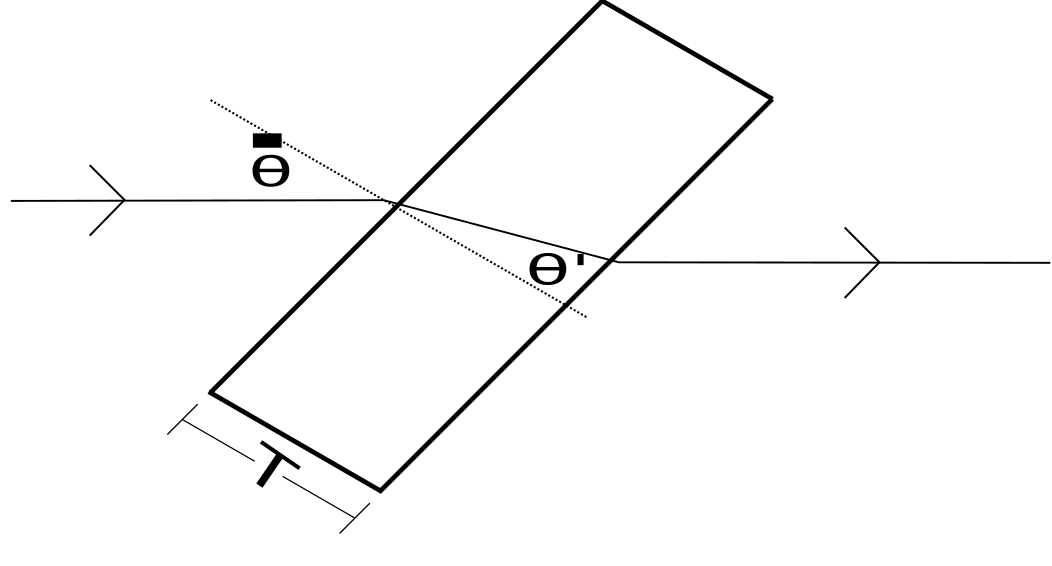
\includegraphics[width=0.75\textwidth]{glasbrech.pdf}
\label{fig:brechglas}
\end{figure}
%
Fällt Licht im Winkel $\Theta$ zum Lot auf eine Glasplatte, 
und schließt der eingetretene Stahl mit dem Lot den Winkel $\Theta'$ ein, 
so kann durch das 
Snelliussche Brechungsgesetz und dem Brechungsindex des Materials n, 
sowie mit der Dicke T der Glasplatte der Phasenunterschied $\phi$ zwischen 
einem Strahl, der am Glas vorbeiläuft und einem, der durch das Glas 
hindurchgeht, errechnet werden. 
Bild~\ref{fig:brechglas} visualisiert die vorliegende Situation.
Es ergibt sich 
Formel~\eqref{eq:glasbrech} für die Phasendifferenz.
\begin{equation}
\Delta\phi(\Theta) = \frac{2\pi}{\lambda_\text{vac}}T\left(
\frac{n-\cos(\Theta - \Theta')}{\cos(\Theta')} - n+1\right)
\label{eq:glasbrech}
\end{equation}
Weitere Rechnung und eine Kleinwinkelnäherung ergibt die einfacherer 
Formel~\eqref{eq:glasbrecheinfach}.
\begin{equation}
\Delta\phi(\Theta) \approx \frac{2\pi}{\lambda_\text{vac}}T\cdot
\frac{n-1}{2n}\Theta^2
\label{eq:glasbrecheinfach}
\end{equation}
In diesem Versuch werden die Anzahl der $2\pi$-Phasenverschiebungen M
der Strahlen während einer Rotation zweier Glasplatten um den Winkel 
$\Theta$ gemessen. Diese Anzahl ergibt sich mit 
Formel~\eqref{eq:glasbrecheinfach} zu
\begin{equation}
M = 2\frac{\Delta\phi}{2\pi} = \frac{2T}{\lambda_\text{vac}}
\frac{n-1}{2n}\Theta^2.
\label{eq:glasfringes}
\end{equation}
Aus dieser Formel kann in diesem Versuch der Brechungsindex n von 
Glasplatten bestimmt werden.\\
\paragraph{Brechindex von Gas}
Durchläuft Licht ein Gas mit dem Brechungsindex n auf einer 
Strecke L, so beträgt der Phasenunterschied zu einem im Vakuum 
laufenden Strahl
\begin{equation}
\Delta\phi = \frac{2\pi}{\lambda_\text{vac}}(n-1)L.
\end{equation}
Hieraus ergibt sich leicht ein Ausdruck für die gezählten 
$2\pi$-Phasenverschiebungen M durch division mit $2\pi$.
Also kann mithilfe von Formel~\eqref{eq:gasfringes} der 
Brechungsindex eines Gases in diesem versuch bestimmt werden.
\begin{equation}
M = \frac{\Delta\phi}{2\pi} = \frac{n-1}{\lambda_\text{vac}}\cdot 2L
\label{eq:gasfringes}
\end{equation}
